\documentclass{beamer}
\newcommand{\myfont}{\rmfamily\normalsize\upshape\mdseries}
\newcommand{\degree}{^\circ}
\newcommand{\R}{\mathbb{R}}
\newcommand{\F}{\mathbb{F}}
\title{\sffamily Review VII(Slides 362 - 443)}
\subtitle{\textbf{Series}\\ }
\institute[UM-SJTU JI]{University of Michigan-Shanghai Jiao Tong University Joint Institute}
\author{Kulu}
\usepackage{graphicx}
\usepackage{picinpar}
\usepackage{indentfirst}
\usepackage{chemformula}
\usepackage{geometry}
\usepackage{subfigure}
\usepackage{appendix}
\usepackage{amsfonts,amsmath,amssymb}
\usepackage{enumerate}
\usepackage{float}
\usepackage{geometry}
\usepackage{latexsym}
\usepackage{listings}
\usepackage{multicol,multirow,multido}
\usepackage{tabularx}
\usepackage{ulem}
\usepackage{tikz}
\usepackage{xcolor}
\usepackage{cite}
\usepackage{setspace}
\usepackage{textpos}
\usepackage{booktabs}
\usepackage{mathtools, nccmath}
\usepackage{hyperref}
\usetheme[dove]{Boadilla}
\usecolortheme{dolphin}
\useoutertheme{miniframes}

\begin{document}
\usebackgroundtemplate{\tikz\node[opacity=0.05]{
        \centerline{
\includegraphics[
                height=\paperheight]{kulu.jpg}}
    };}
\begin{titlepage}
    \begin{center}
        VV186 - Honors Mathmatics II
    \end{center}
\end{titlepage}
\myfont


\section{Series}


\begin{frame}
    \frametitle{Series}
    \hspace{1em}
    Let $(a_n)$ be a sequence in a normed vector space $(V, ||\cdot||)$.
    We define $s_n:= \sum_{k=0}^n a_k$  as the \textbf{n-th partial sum} of $(a_n)$.
    We say that $(a_n)$ is \textbf{summable} with sum $s \in V$ if $\underset{n\to\infty}{\lim}⁡ s_n=s$.
    We use $\sum_{k=0}^\infty a_k$  , or $∑a_k$ to denote s as well as
    the "procedure of summing the sequence $(a_n)$",
    and call this notation \textbf{infinite series}.
    \\
    \vspace{1em}
    Comment. While the definition of series is in general vector space, we will focus on real series and real function series later on.
\end{frame}

\begin{frame}
    \frametitle{Cauchy Criterion}
    \hspace{1em}
    Generally, a closed form sum of a sequence is hard to find. Instead, we
    will mostly focus on whether the series converges.
    The starting point will be the \textbf{Cauchy Criterion}(Slides 380):\\
    \hspace{1em}Let $\sum a_k$ be a sequence in a complete vector space $(V, ||\cdot||)$ Then
    \begin{align*}
        \sum a_k \text{ converges}
         & \Leftrightarrow (s_n ) \text{ converges}                                                                                              \\
         & \Leftrightarrow (s_n) \text{ is Cauchy}                                                                                               \\
         & \Leftrightarrow \forall \varepsilon>0, \exists N \in \mathbb{N} ~\text{such that}~ \forall m,n>N, ||s_m-s_n ||<\varepsilon            \\
         & \Leftrightarrow \forall \varepsilon>0, \exists N \in \mathbb{N}~ \text{such that}~ \forall m>n>N, ||\sum_{k=n+1}^m a_k ||<\varepsilon
    \end{align*}
    Two important colloaries are:
    \begin{itemize}
        \item  If $(a_n)$ is summable, $a_n\to 0$ as $n\to \infty$
        \item  If $(a_n)$ is summable, $\sum_{k=n}^\infty a_k\to 0$ as $n \to \infty$
    \end{itemize}
\end{frame}




\begin{frame}
    \frametitle{Tests for Convergence}
    \hspace{1em}
    A number of tests (for series of positive real numbers) are given
    throughout the slides:
    \begin{itemize}
        \item 1. The Comparison Test (P392, 3.5.15)
        \item 2. The Root Test (P401, 3.5.22)
        \item 3. The Root Test in Limits Form (P405, 3.5.26)
        \item 4. The Ratio Test (P407, 3.5.28)
        \item 5. The Ratio Test in Limits Form (P410, 3.5.30)
        \item 6. The Ratio Comparison Test (P411, 3.5.31)
        \item 7. Raabe’s Test (P413, 3.5.32)
        \item 8. Leibniz Theorem (P413, 3.5.38)
    \end{itemize}
\end{frame}

\begin{frame}
    \begin{figure}[htbp]
        \centering
        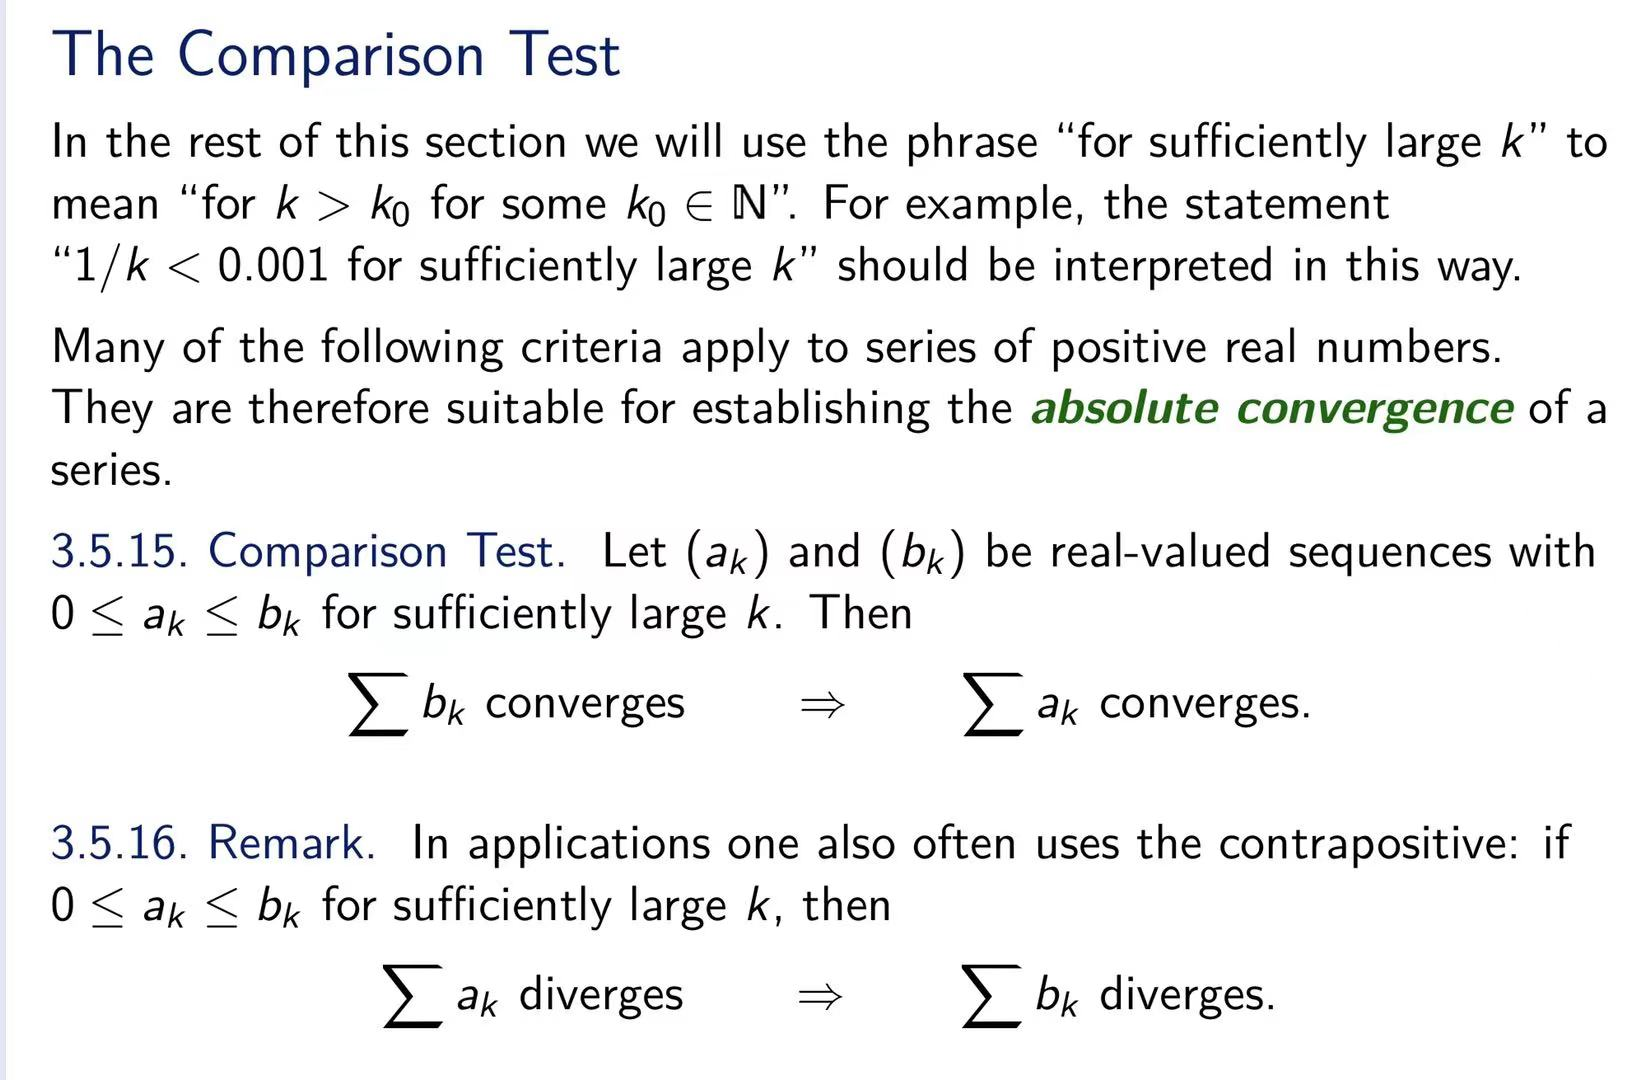
\includegraphics[width=12cm]{comparison.jpg}
    \end{figure}
\end{frame}

\begin{frame}
    \begin{figure}[htbp]
        \centering
        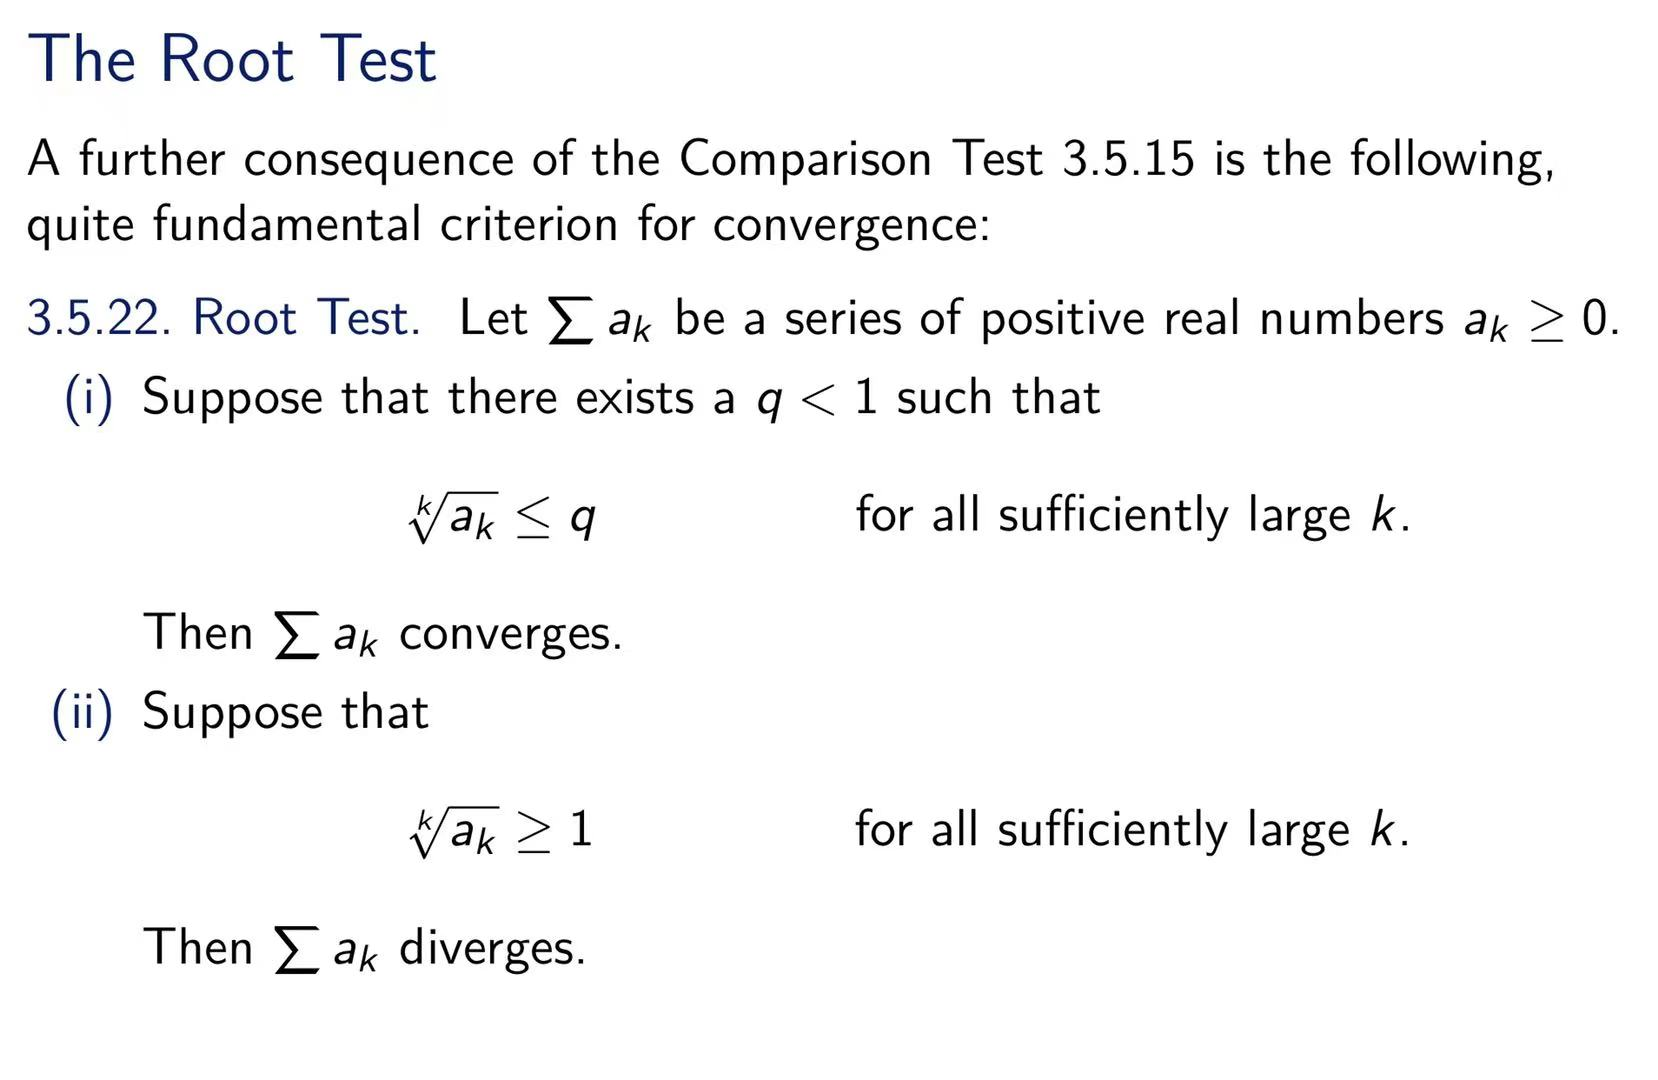
\includegraphics[width=12cm]{root.jpg}
    \end{figure}
\end{frame}
\begin{frame}
    \begin{figure}[htbp]
        \centering
        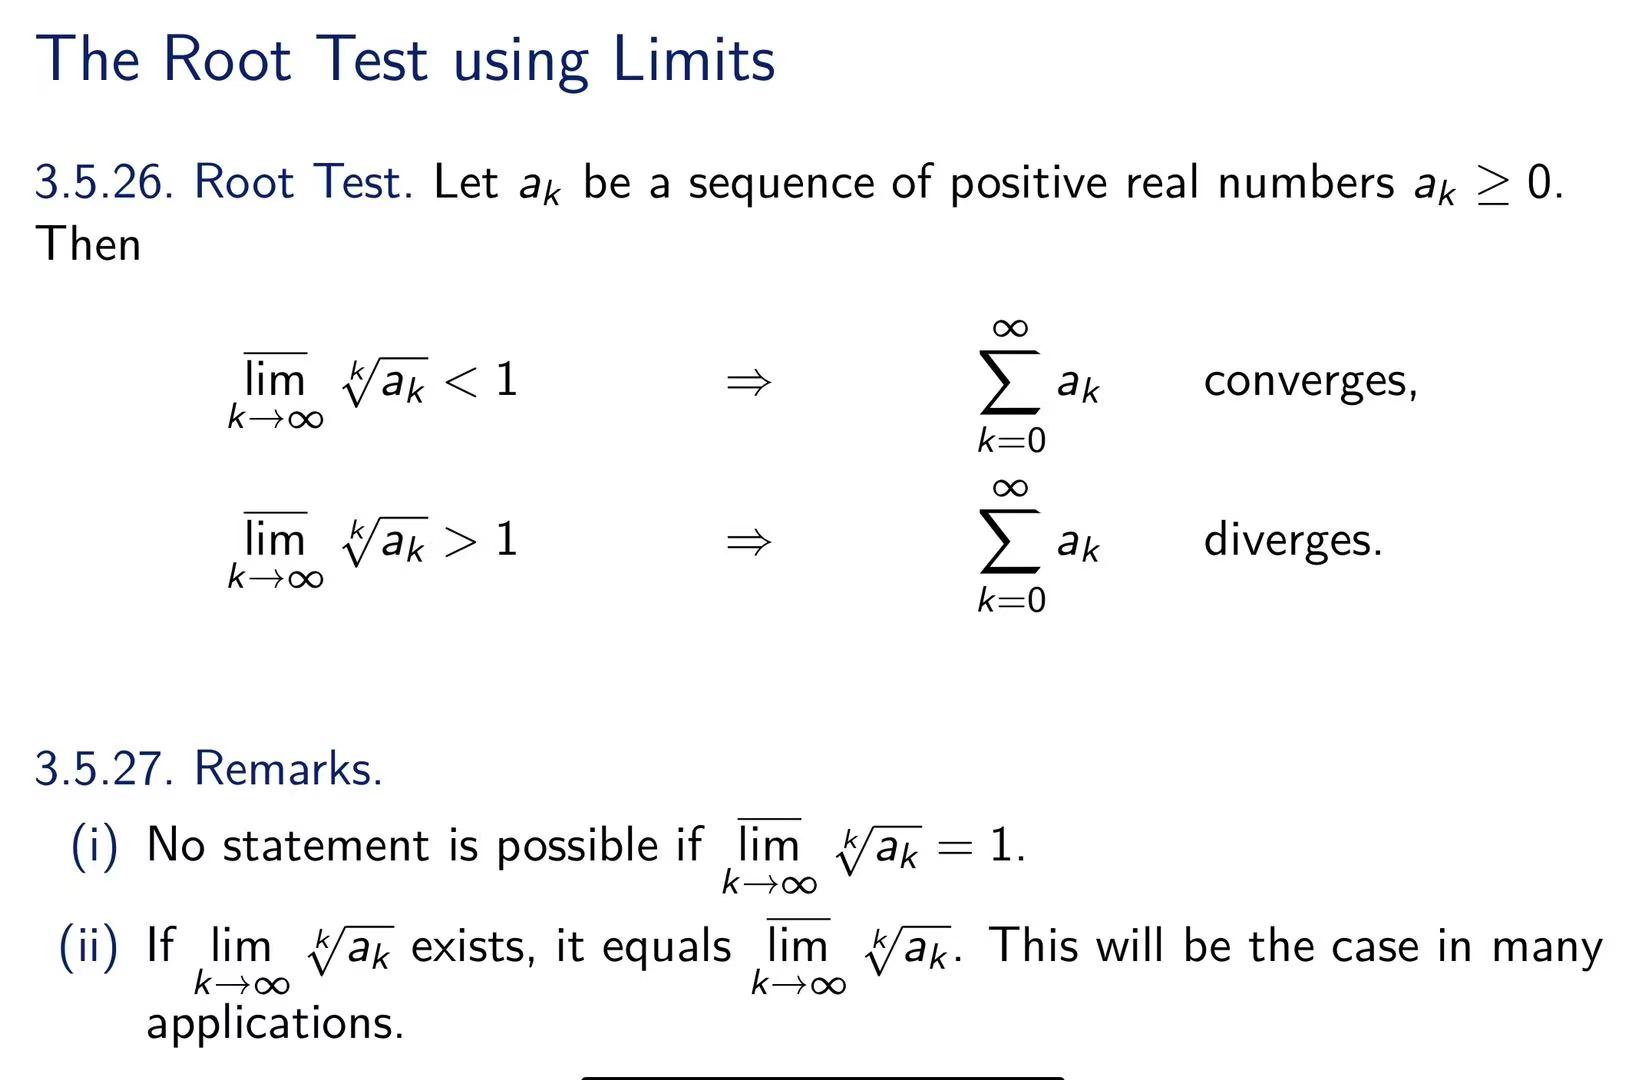
\includegraphics[width=12cm]{root_limit.jpg}
    \end{figure}
\end{frame}

\begin{frame}
    Prove that the series $\sum a_m=\frac{1}{2}+\frac{1}{3}+\frac{1}{2^2}+\frac{1}{3^2}+\frac{1}{2^3}+\frac{1}{3^3}+...$ is convergent.

\end{frame}

\begin{frame}
    \begin{figure}[htbp]
        \centering
        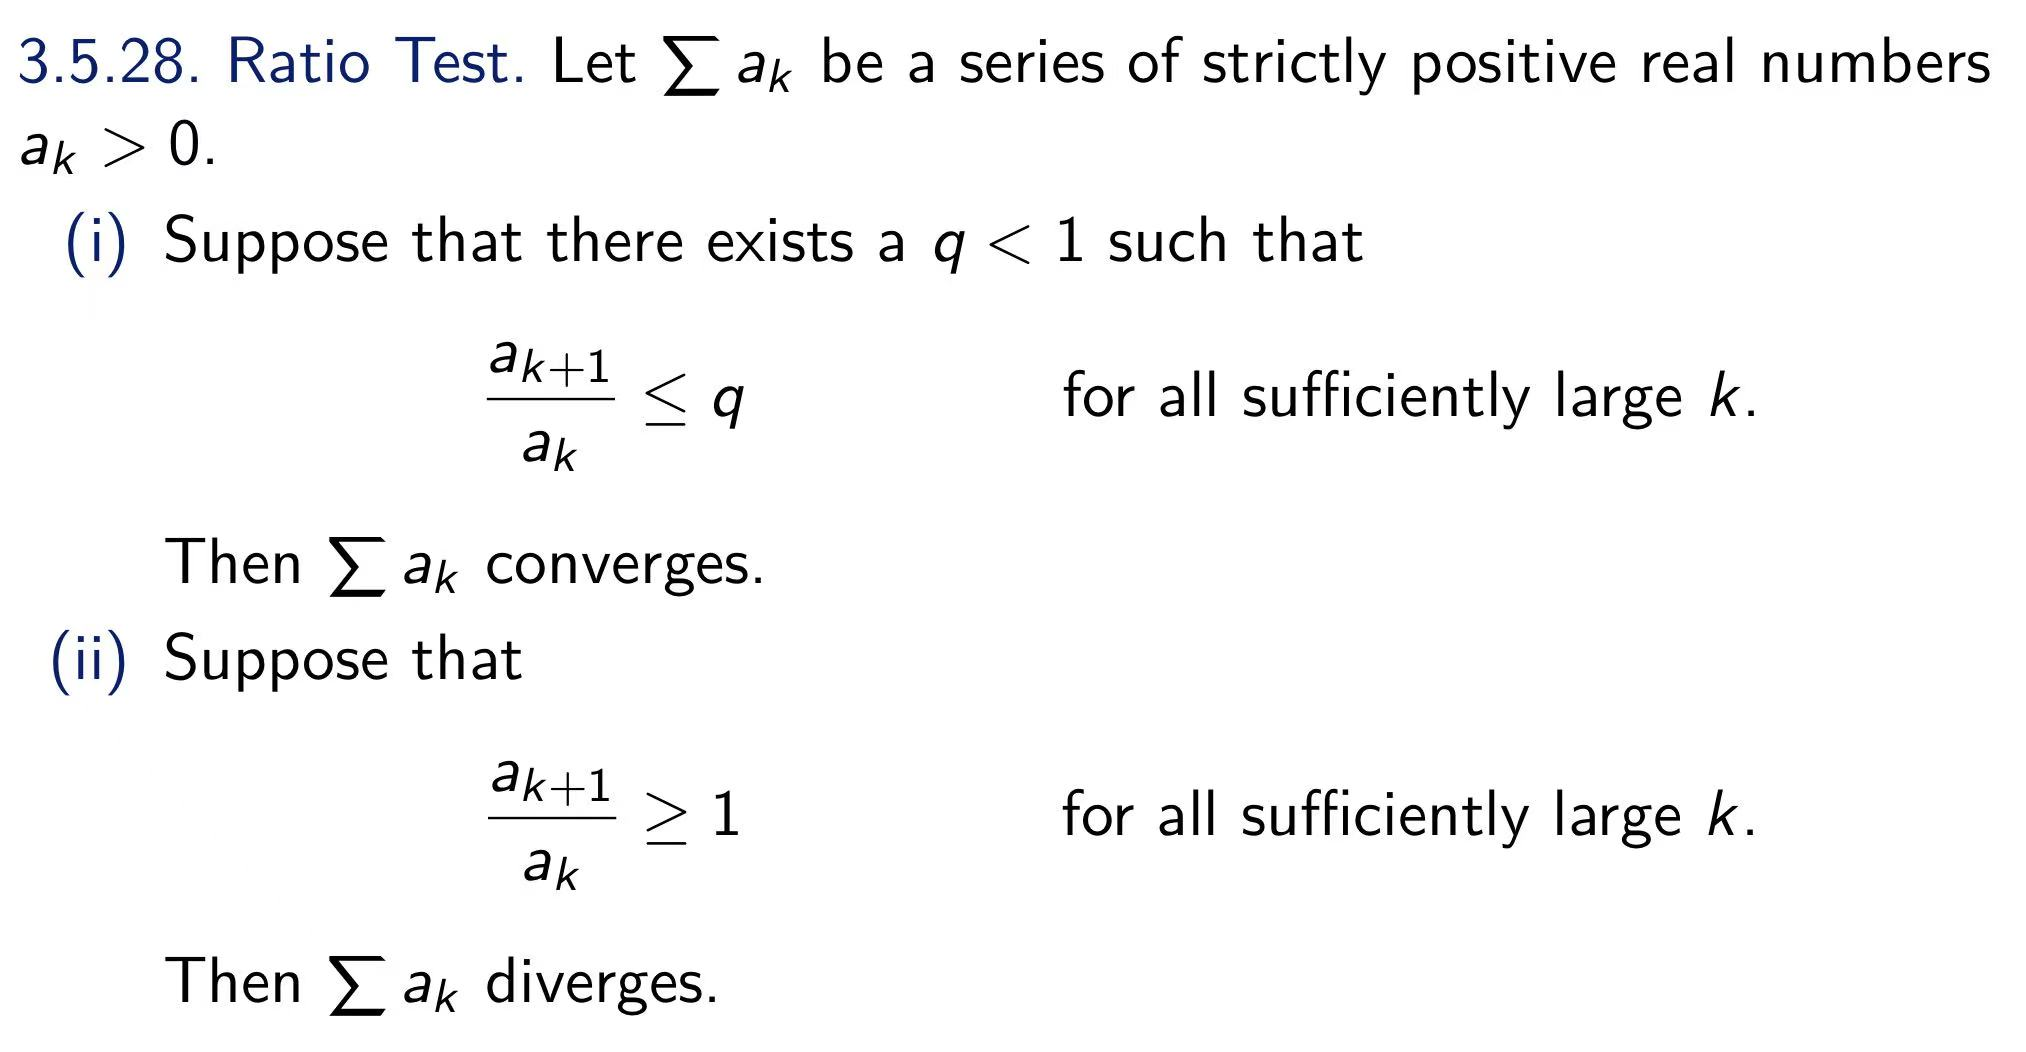
\includegraphics[width=12cm]{ratio.jpg}
    \end{figure}
\end{frame}

\begin{frame}
    \begin{figure}[htbp]
        \centering
        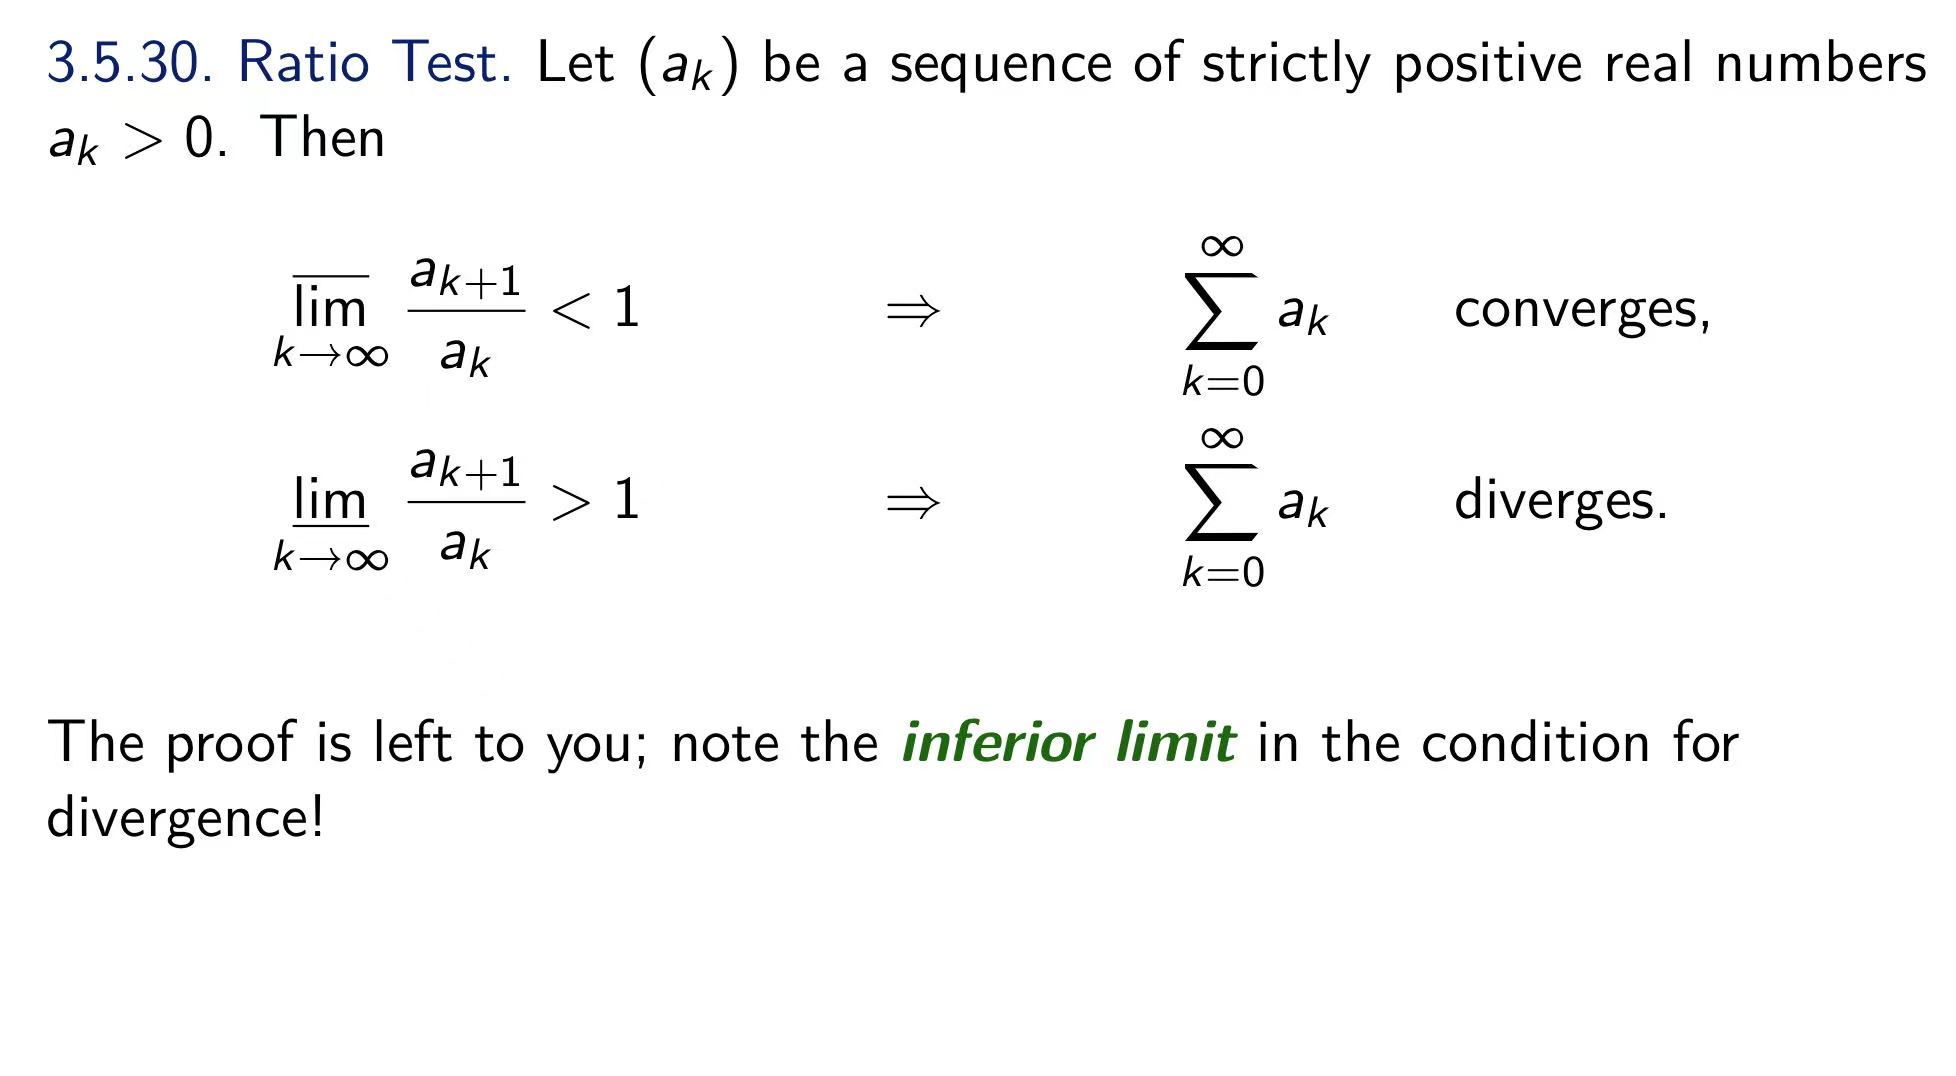
\includegraphics[width=12cm]{ratio_limit.jpg}
    \end{figure}
\end{frame}
\begin{frame}
    \begin{figure}[htbp]
        \centering
        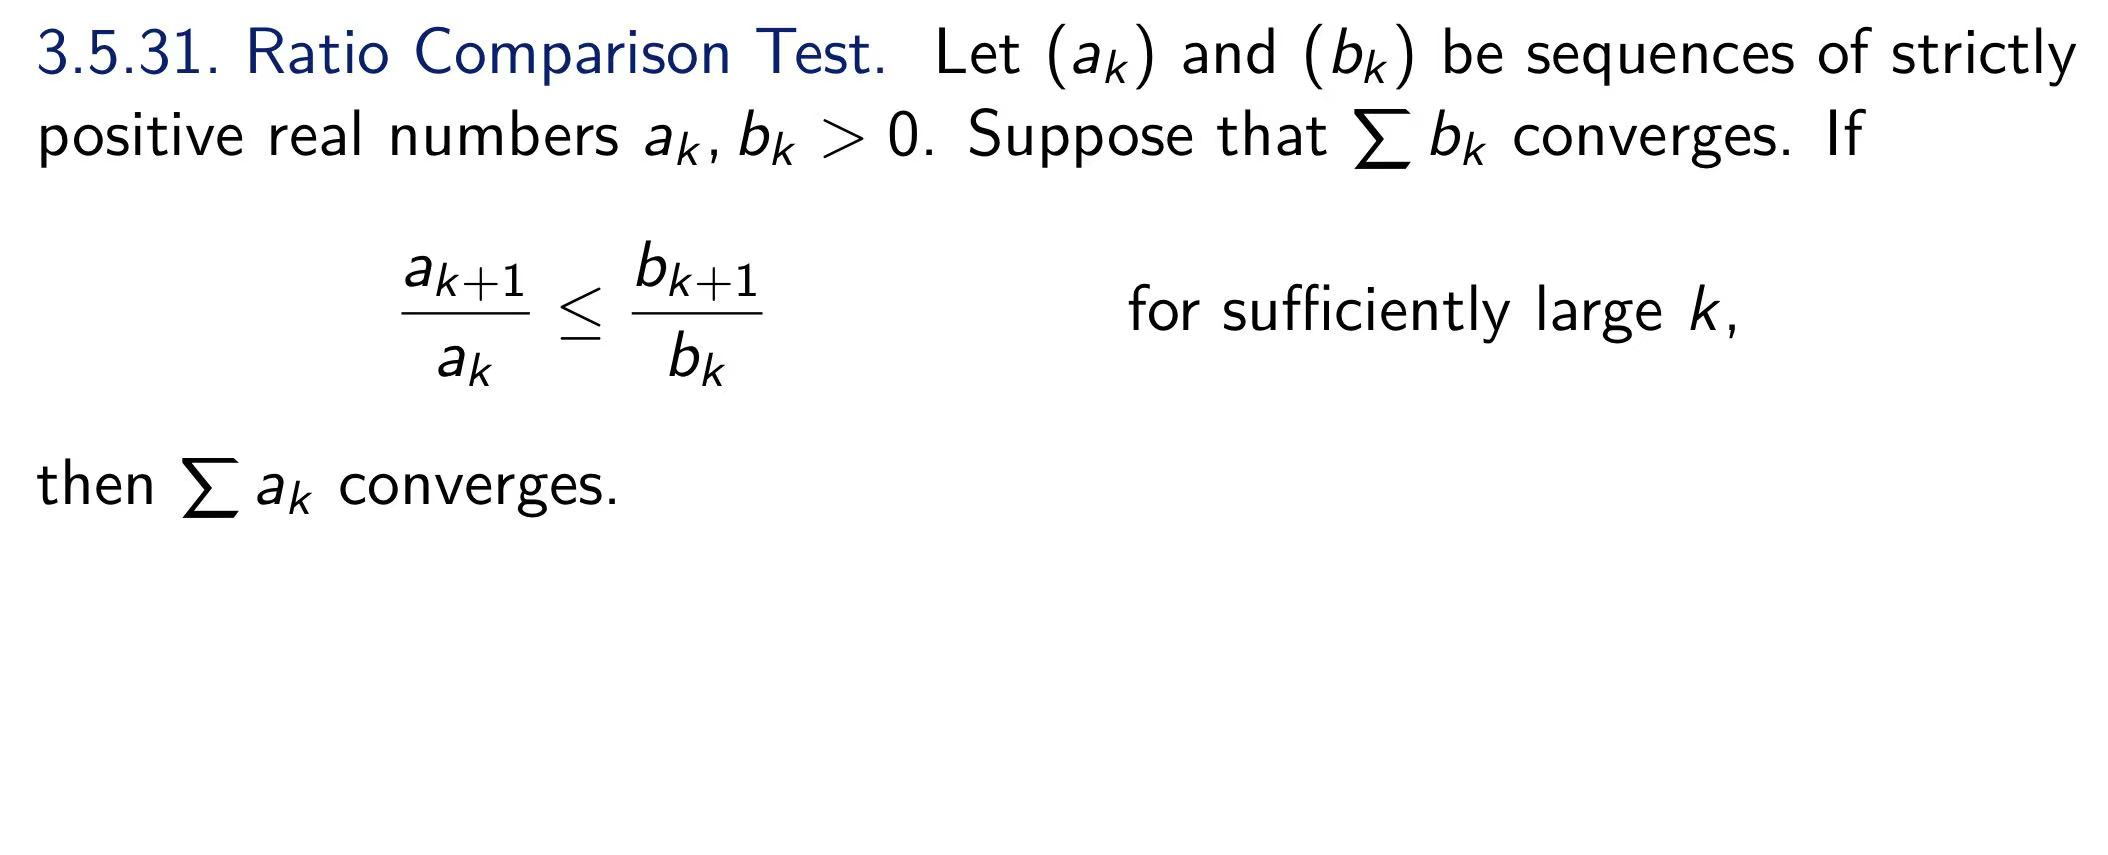
\includegraphics[width=12cm]{ratiocompare.jpg}
    \end{figure}
\end{frame}
\begin{frame}
    \begin{figure}[htbp]
        \centering
        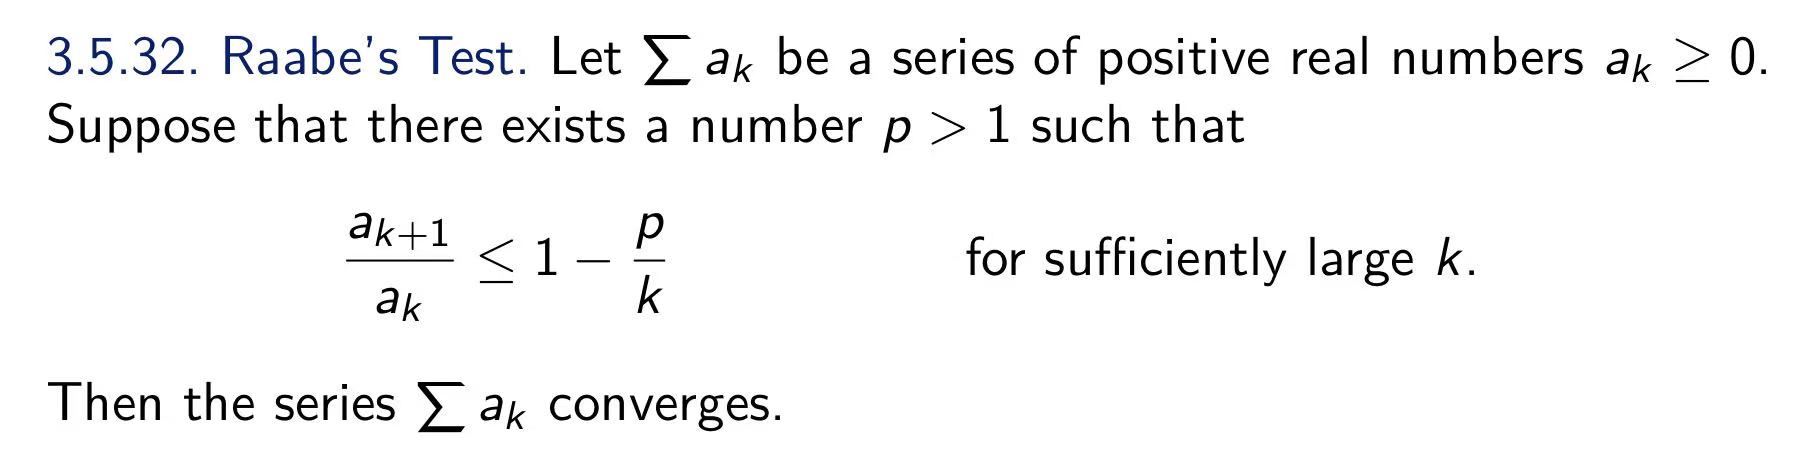
\includegraphics[width=12cm]{raabe.jpg}
    \end{figure}
\end{frame}
\begin{frame}
    \begin{figure}[htbp]
        \centering
        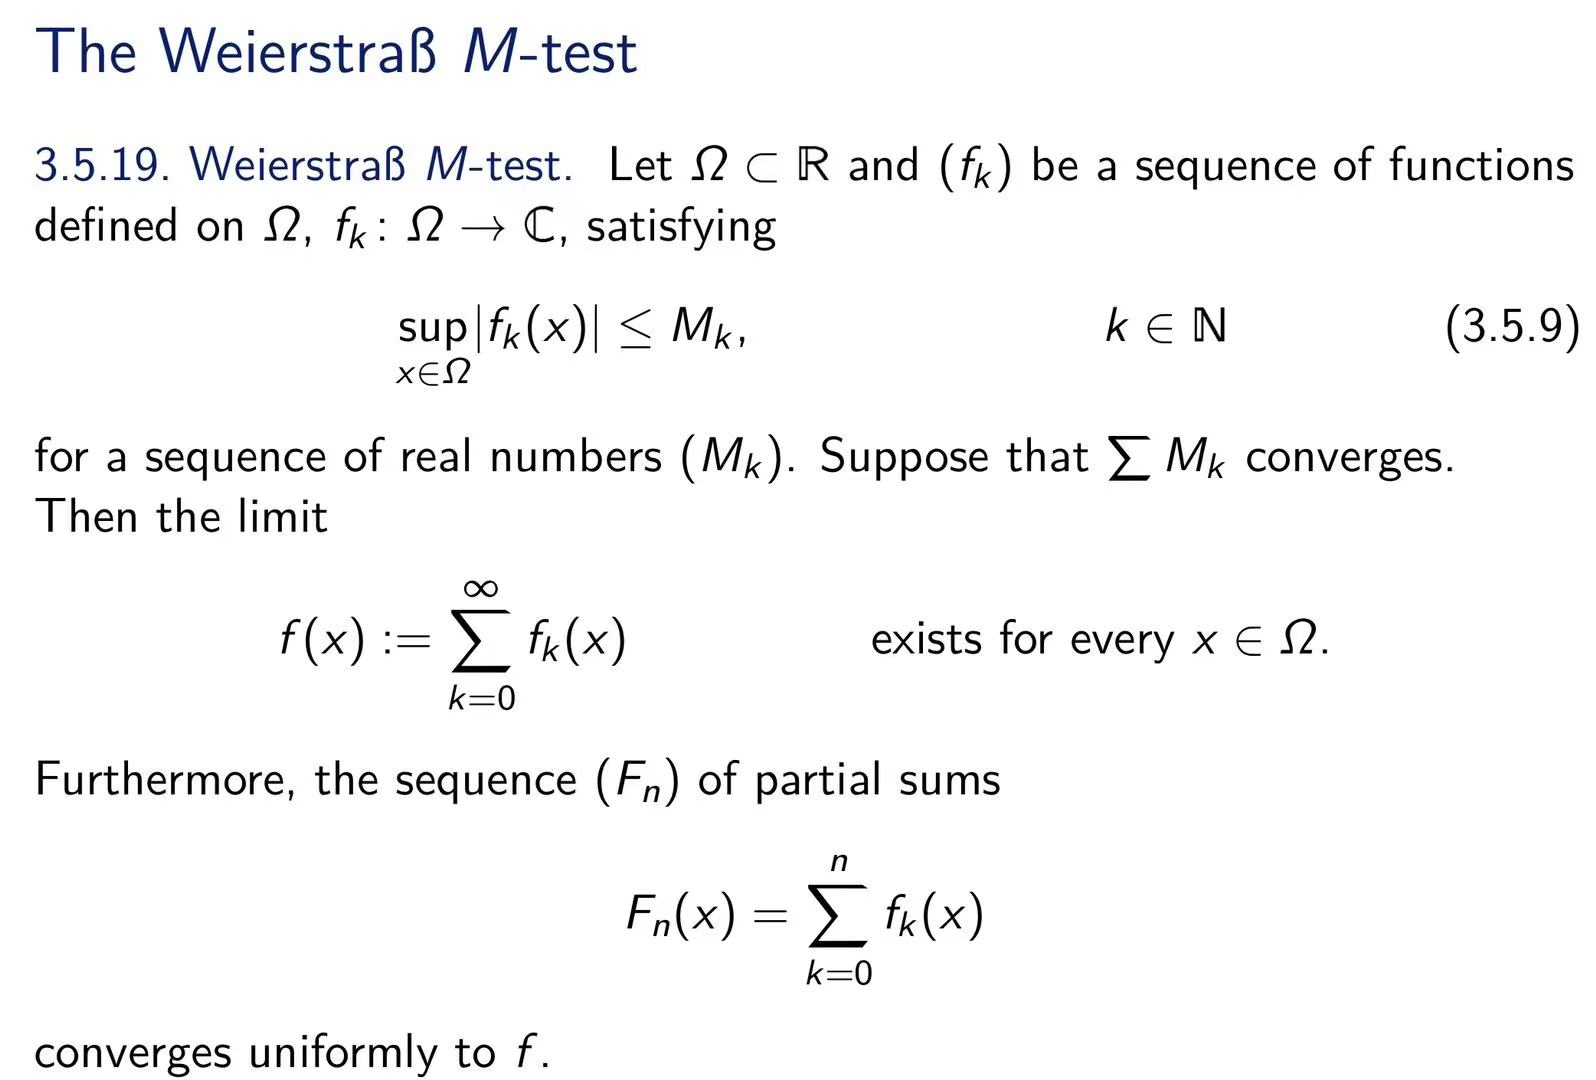
\includegraphics[width=12cm]{w.jpg}
    \end{figure}
\end{frame}
\begin{frame}
    \begin{figure}[htbp]
        \centering
        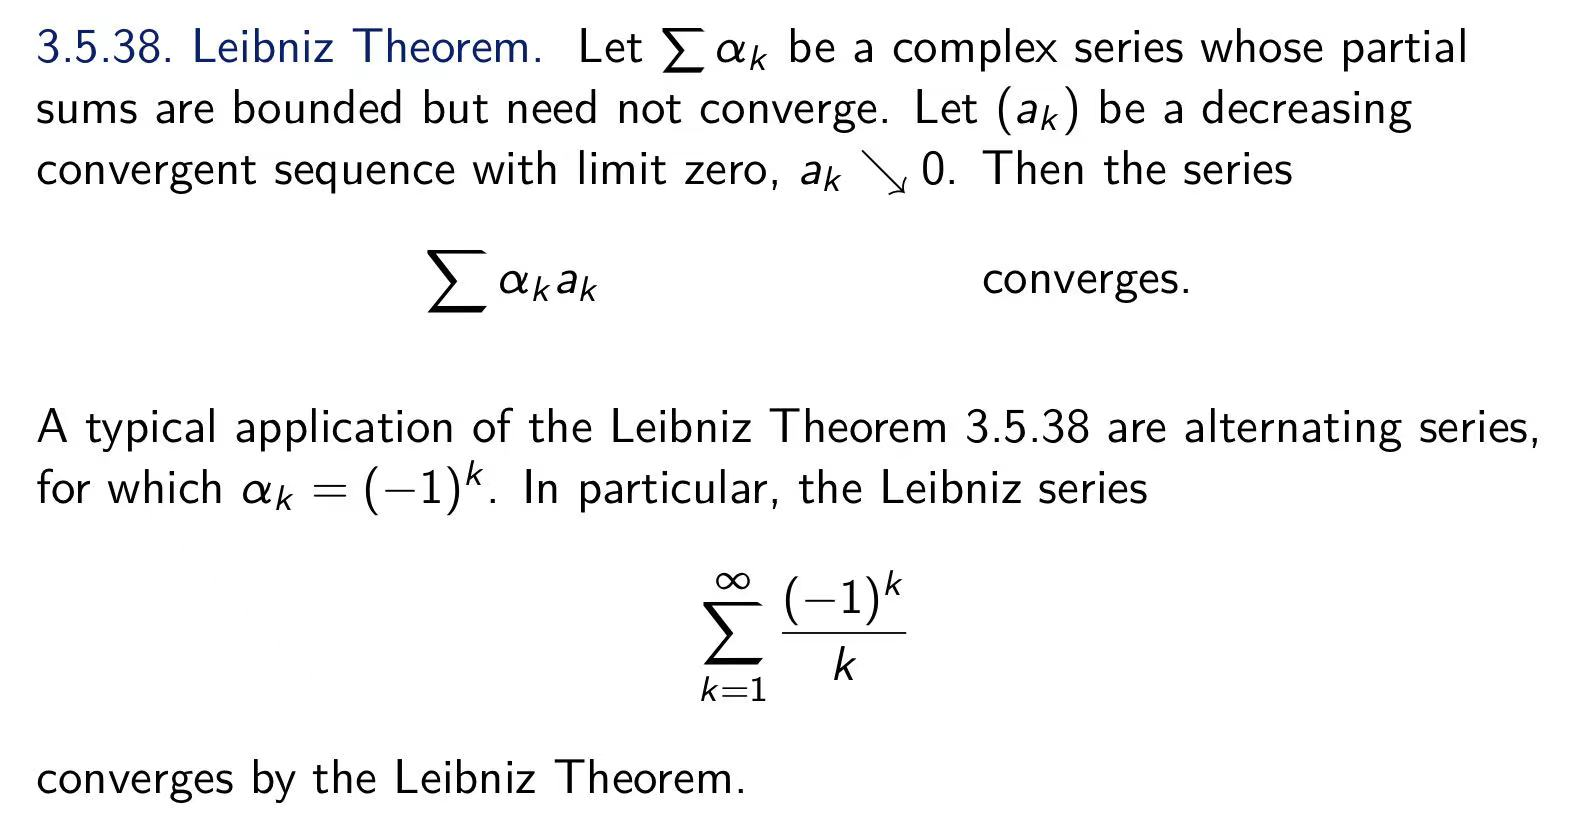
\includegraphics[width=12cm]{l.jpg}
    \end{figure}
\end{frame}
\begin{frame}
    \frametitle{Procedure of Determining Convergence}
    \hspace{1em}We rank the "usefulness" of all these tests as follows:
    \begin{center}
        \begin{itemize}
            \item[] Cauchy Criteria
            \item[>] Comparison Test
            \item[>] Ratio Test (in Limits)
            \item[>] Root Test (in Limits)
            \item[>] Ratio Comparison Test/Raabe’s Test...
        \end{itemize}
    \end{center}
    \par
    \hspace{1em}
    When you are asked to determine whether a series converges, it’s
    recommended to use the tests in this order. Thus if you have a hard time
    memorizing all the tests, do first memorize the more "important" tests.

\end{frame}

\begin{frame}
    \frametitle{Exercises}
    Suppose $\sigma > 0$, $a_n > 0$, prove that:

    (1) If $\forall$n>N, $(\ln \frac{1}{a_n})(\ln n)^{-1}\geq 1+\sigma$, then $\sum_{n=1}^\infty a_n$ converges

    (2) If $\forall$n>N, $(\ln \frac{1}{a_n})(\ln n)^{-1}\leq 1$, then $\sum_{n=1}^\infty a_n$ diverges
\end{frame}

\begin{frame}
    \frametitle{Exercises}
    1. Please determine whether the following series converge or not!
    \begin{itemize}
        \item $$\sum_{n=0}^\infty \frac{4n(n+2)!}{(2n)!}$$
        \item $$\sum_{n=1}^\infty \frac{\sin(n\theta)}{n^2} \text{, where } \theta \text{ is fixed}$$%∑2_nϵℕ▒(sin⁡(nθ))/n^2 , where θ is a fixed number
        \item $$\sum_{n=0}^\infty \frac{(2n)!}{4^n (n+1)!n!} \text{ (Hint: This appears in the slides!)}$$%∑_𝑛𝜖ℕ▒((2𝑛)! )/(4^𝑛 (𝑛+1)!𝑛!) 
        \item $$\sum_{n=2}^\infty \frac{1}{(\ln n)^{(\ln n)}}$$%∑2_nϵℕ▒1/(ln⁡n )^ln⁡n   (SJTU Math textbook, P13) 
    \end{itemize}
\end{frame}
\begin{frame}
    \frametitle{Exercises}
    2. Prove the \textbf{limit comparison test}:\\
    \vspace{1em}
    For two positive series $\sum a_n$ and $\sum b_n$, if
    $$0< \underset{n \to \infty}{\lim} \frac{a_n}{b_n}< \infty $$
    then $a_n$ and $b_n$ both converges or diverges.

\end{frame}
\begin{frame}
    \frametitle{Exercises}
    3. Prove that if a positive series $a_n$ diverges, then

    (1) $\sum \frac{a_n}{1+a_n}$ diverges.

    (2) $\sum \frac{a_n}{1+n^2a_n}$ converges.
\end{frame}
\begin{frame}
    \frametitle{Absolute and Conditionally Convergence}
    \hspace{1em}
    \begin{itemize}
        \item A series $\sum a_n$ is called \textbf{absolutely convergent} if $\sum ||a_n||$ converges.
        \item If $\sum a_n$ converges while $\sum ||a_n||$ doesn’t, than it’s called \textbf{conditionally convergent}.
        \item In a complete vector space (which is the case in our cases), absolutely
              convergent implies convergent.
    \end{itemize}
    To test for conditionally convergence, we have the following theorem:
    \hspace{1em}Let $\sum \alpha_k$ be a complex series whose partial sum are bounded but need not converge.
    Let $(a_k)$ be a decreasing convergent sequence with limit zero, then the series $\sum \alpha_k a_k$ converges (Slide 418)
    \\ \vspace{1em}
    Comment. With this result, it is easy to see that $\sum_{k=1}^\infty \frac{(-1)^k}{k}$ converges

\end{frame}

\begin{frame}
    \begin{figure}[htbp]
        \centering
        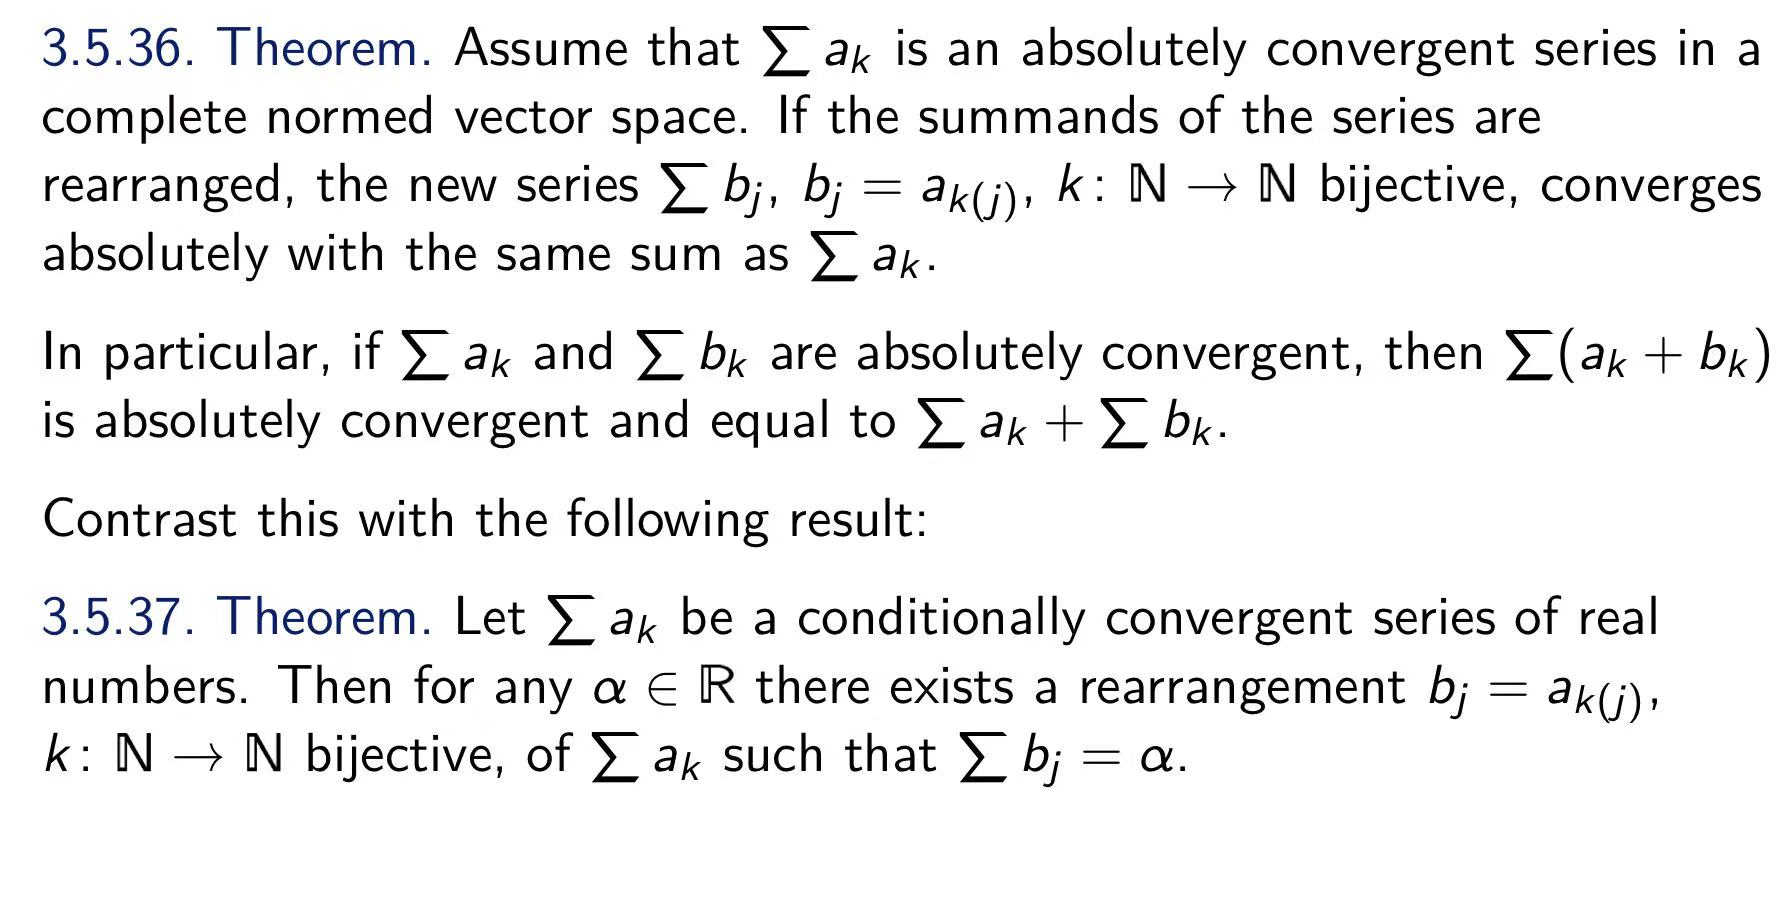
\includegraphics[width=12cm]{rearrange.jpg}
    \end{figure}
\end{frame}

\begin{frame}
    \begin{figure}[htbp]
        \centering
        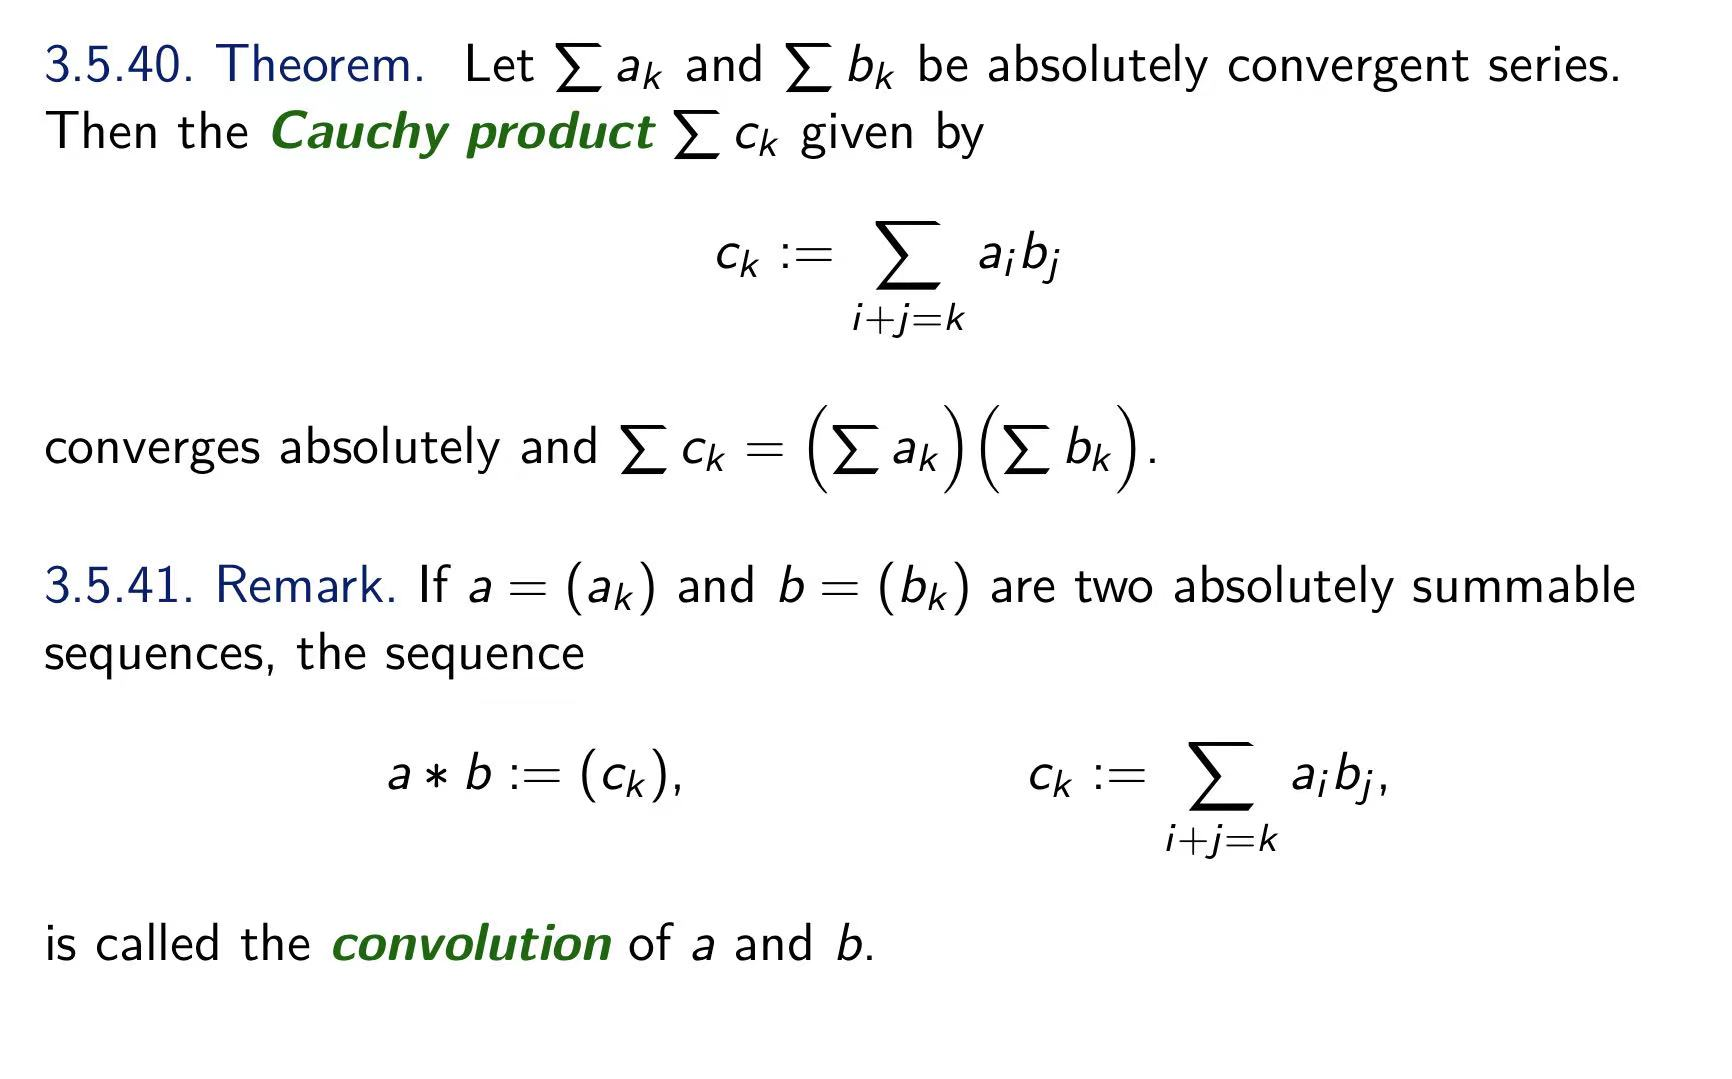
\includegraphics[width=12cm]{convolution.jpg}
    \end{figure}
\end{frame}

\section{Power Series}
\begin{frame}
    \frametitle{Power Series}

    \hspace{1em} Of all function series, one useful kind is the \textbf{power series},
    which is the infinite sum of monomials.
    $$\sum_{k=0}^\infty a_k z^k \text{ or simply } \sum a_k z_k$$
    \hspace{1em} We call this \itshape formal \myfont as we are yet to find whether the series converge or
    not for given $z$.\\
    \vspace{1em}
    We can add and multiply two power series:
    \begin{itemize}
        \item $\sum a_n z^n +\sum b_n z^n = \sum (a_n+b_n) z^n$
        \item $\sum a_n z^n \cdot \sum b_n z^n = \sum (a*b)_n z^n$
    \end{itemize}
    \href{https://www.zhihu.com/question/54677157}{\textcolor{red}{\textbf{Why convolution?}}}
\end{frame}
\begin{frame}
    \frametitle{Raduis of Convergence}
    \hspace{1em} Let $\sum a_k z^k$ be a complex power series.
    Then there exists a unique number $\rho \in (0, +\infty)$ such that
    \begin{itemize}
        \item[i)] the power series $\sum a_k z^k$ is absolutely convergent at $z_0  \in \mathbb{C}$ if $|z_0 |<\rho$;
        \item[ii)] the power series diverges at $z_0  \in \mathbb{C}$ if $|z_0 |>\rho$
    \end{itemize}
    \vspace{1em}
    Hadamard's formula:
    $$\rho=\frac{1}{\underset{k\to \infty}{\varlimsup} \sqrt[k]{|a_k|}}$$
    where $\rho$ is called the radius of convergence, if we informally write $1/\infty = 0, 1/0 = \infty$.

\end{frame}
\begin{frame}
    \frametitle{Remarks}
    \begin{itemize}
        \item For a complex power series, the set of z which the series converge
              will always be a circle. For a real power series, the set will be a line
              segment and the radius of convergence is one half of the length.
        \item We can’t say much if we have $|z| = \rho$. The series may converge or
              diverge or conditionally converge.
    \end{itemize}
    \vspace{1em}
    Do check for the boundary!
    \begin{figure}
        \centering
        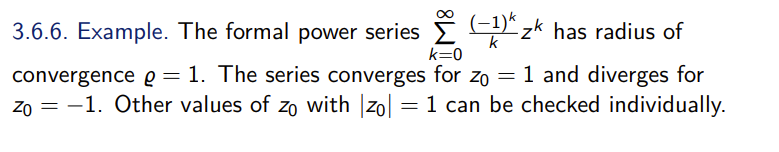
\includegraphics[width=1\textwidth]{boundary.png}
    \end{figure}
\end{frame}
\begin{frame}
    \frametitle{Exercise}
    5. Decide for the following real power series, on which interval would it
    converge?
    \vspace{1em}
    \begin{itemize}
        \item $$\sum_{n=1}^\infty \frac{(x-1)^n}{2^n n}$$
        \item $$\sum_{n=1}^\infty \frac{x^{2n}}{n-3^{2n}}$$
    \end{itemize}
\end{frame}

\begin{frame}
    \frametitle{Abel Theorem}
    (1) If a power series is convergent at x=$x_0$, then it is absolutely convergent for $|x|<|x_0|$;

    (2) If a power series is divergent at x=$x_0$, then it is divergent for $|x|>|x_0|$.
\end{frame}

\begin{frame}
    \begin{figure}[htbp]
        \centering
        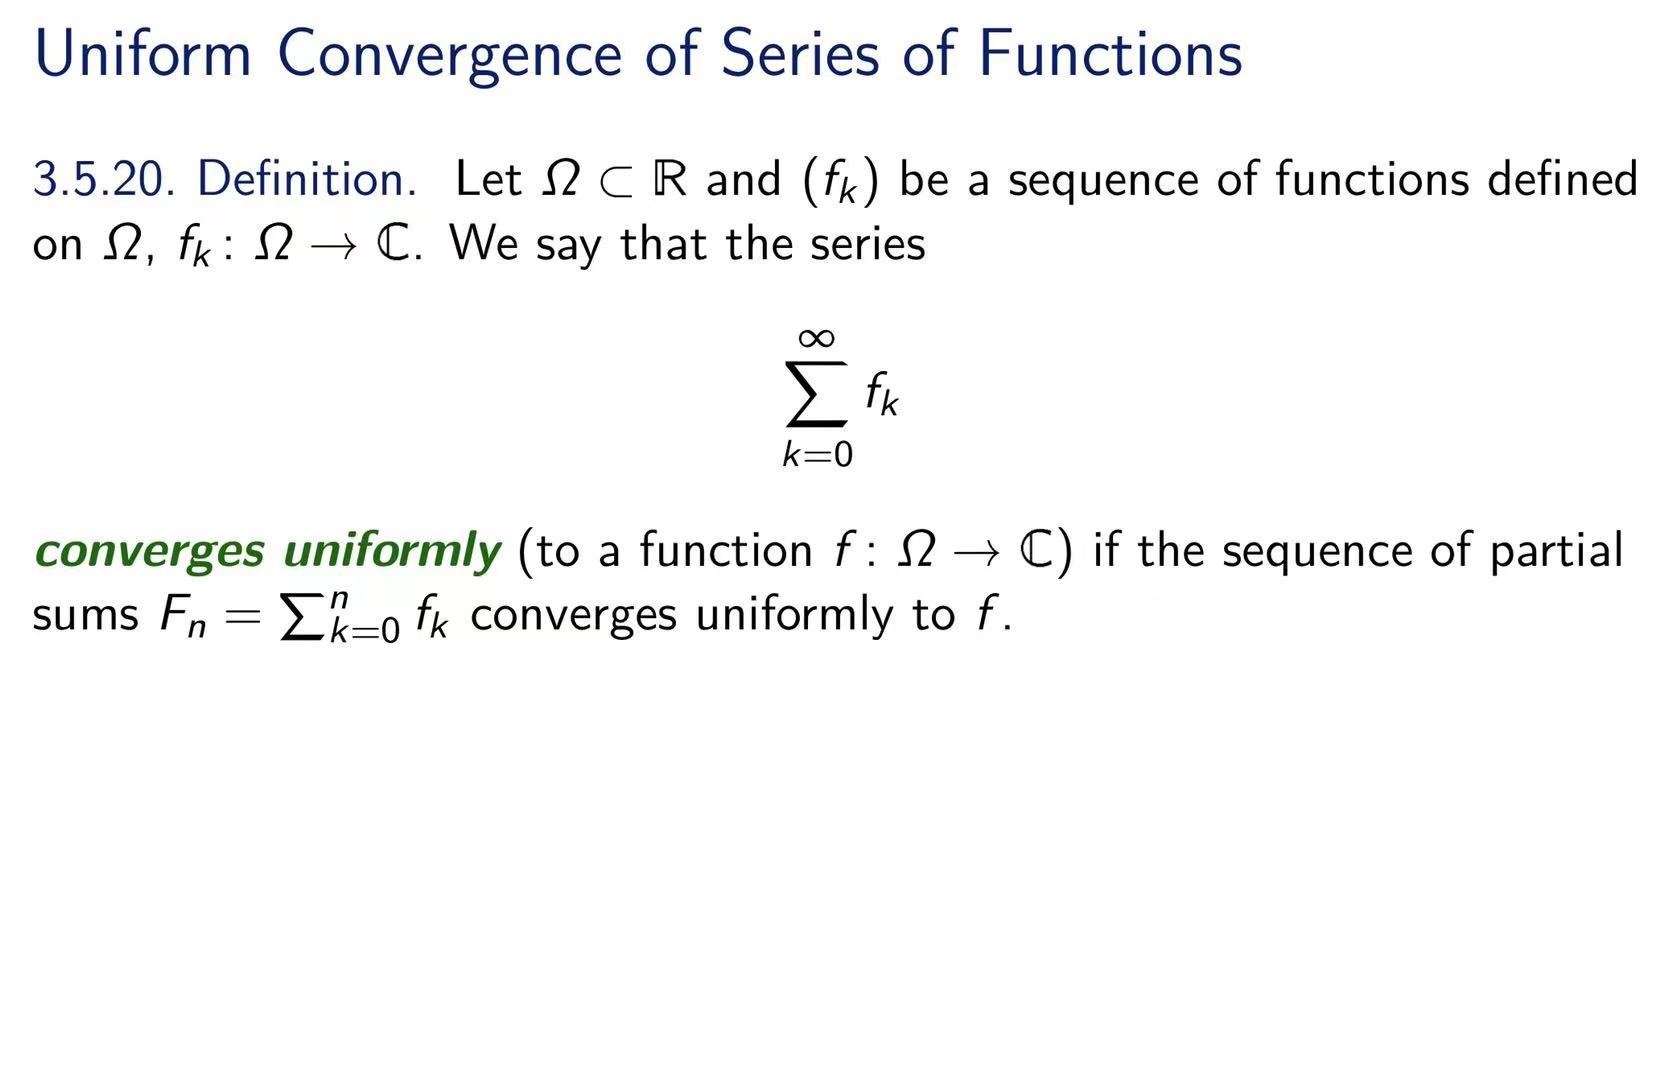
\includegraphics[width=12cm]{uniform_converge.jpg}
    \end{figure}
\end{frame}

\begin{frame}
    \begin{figure}[htbp]
        \centering
        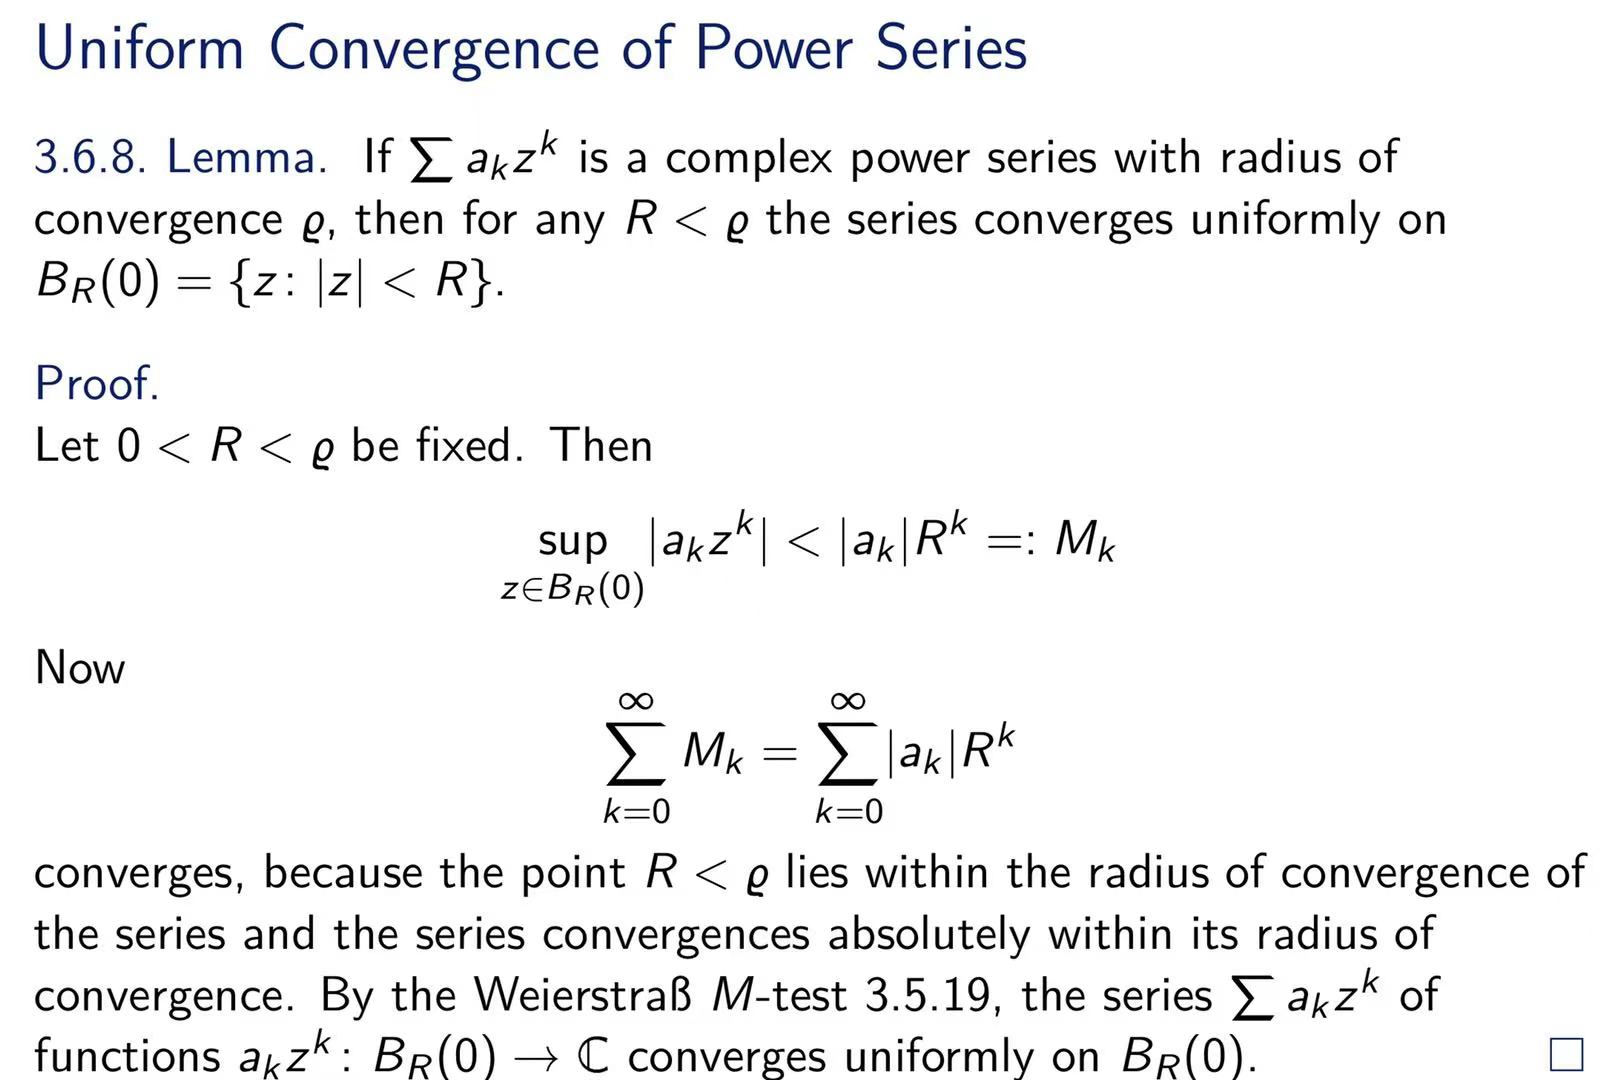
\includegraphics[width=12cm]{uniform_converge2.jpg}
    \end{figure}
\end{frame}

\begin{frame}
    \begin{figure}[htbp]
        \centering
        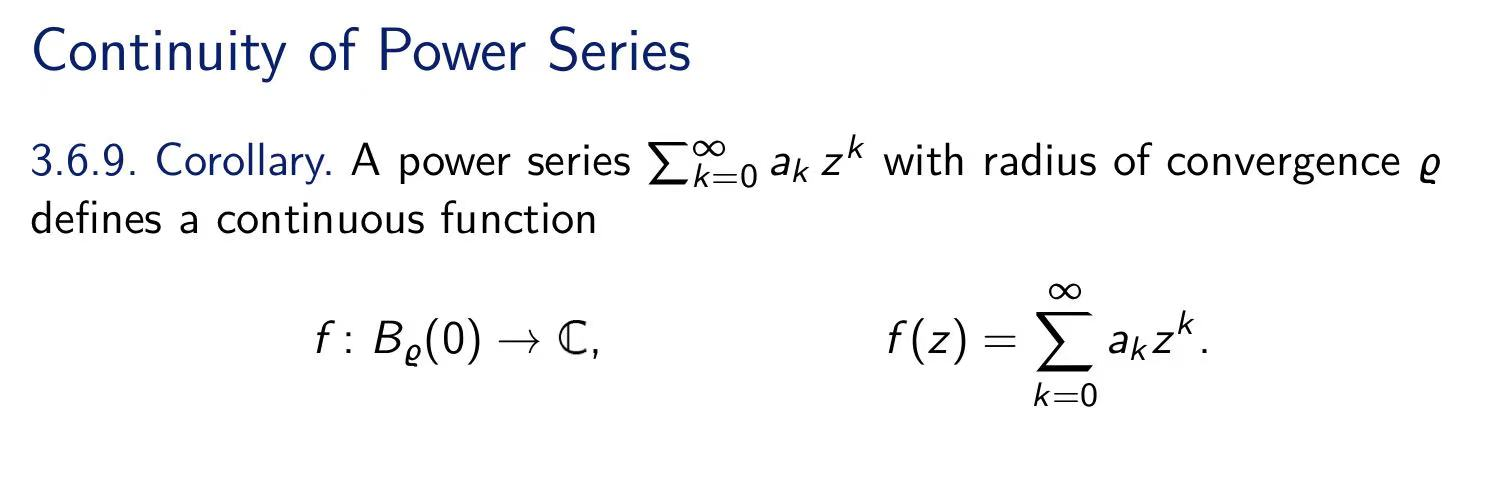
\includegraphics[width=12cm]{continuity.jpg}
    \end{figure}
\end{frame}

\begin{frame}
    \frametitle{Differentiability of Power Series}
    \hspace{1em}
    The power series $\sum a_k z^k$ with radius of convergence $\rho$
    defines a differentiable function $f : B_\rho(0) \to \mathbb{C}$. Furthermore,
    $$f~'(z_0)=\sum k a_k z_0^{k-1}$$
    Remarks:
    \begin{itemize}
        \item[1.] This means that we can differentiate a power series ”term by term”
            inside the radius of convergence.
        \item[2.] Recursively apply this theorem to see that any power series is
            infinitely differentiable inside its radius of convergence. In fact, for a
            function to be expressable as a power series (which we call it
            \textbf{analytic}) is stronger than being infinitely differentiable. (You will
            learn more about this in Vv286!)
    \end{itemize}
\end{frame}





\section{Appendix}



\begin{frame}
    \frametitle{Reference}
    \begin{itemize}
        \item 2021-Vv186 TA-Niyinchen
    \end{itemize}
\end{frame}
\begin{frame}
    \frametitle{End}
    \centering
    \LARGE{Thanks!}


\end{frame}
\end{document}